\documentclass[12pt, oneside]{report}

\pdfcompresslevel=0
\pdfobjcompresslevel=\pdfcompresslevel

\usepackage[letterpaper, scale=0.92, centering]{geometry}
\usepackage{amssymb,amsmath,pifont,amsfonts,comment,enumerate}
\usepackage{currfile,xstring,hyperref,tabularx,graphicx,wasysym}
\usepackage{caption}
\usepackage[dvipsnames,table]{xcolor}
\usepackage{multicol,multirow,array,listings,tabularx,lastpage,textcomp,booktabs}

\usepackage{enumitem}
\usepackage{subcaption}
\usepackage{minted}
\usepackage{bookmark}

\setlength{\parindent}{0em}
\setlength{\parskip}{1em}

\hypersetup{
    colorlinks=true,
    linkcolor=black,%blue,
    filecolor=black,%magenta,      
    urlcolor=black,%cyan,
    pdftitle={Sharelatex Example},
    pdfpagemode=FullScreen
}

\captionsetup{hypcap=false}

\newcommand{\review}[0]{\textcolor{red}{REVIEW THIS}}
\newcommand{\chap}[1]{\chapter*{#1}\addcontentsline{toc}{chapter}{#1}}
\newcommand{\sect}[1]{\section*{#1}\addcontentsline{toc}{section}{#1}}
\newcommand{\subsect}[1]{\subsection*{#1}\addcontentsline{toc}{subsection}{#1}}
\newcommand{\subsubsect}[1]{\subsubsection*{#1}\addcontentsline{toc}{subsubsection}{#1}}


\title{ECE 157C/272C HW 01}
\author{Caleb Harris}
\date{}

\begin{document}
\graphicspath{ {./graphics} }

\begin{titlepage}
    \centering
    \pagenumbering{gobble}
    \maketitle
    \tableofcontents
    % \listoffigures
    % \listoftables
\end{titlepage}
\pagenumbering{arabic}


% ============================================================
\chap{Setup and Execution}
% ============================================================

\sect{Dependencies}

The project requires Python 3.10 or later. All dependencies are listed in \texttt{requirements.txt} and can be installed with:

\begin{minted}{bash}
pip install -r requirements.txt
\end{minted}

The key packages are:

\begin{itemize}
    \item \texttt{openai>=1.30.0} --- LLM API client
    \item \texttt{langgraph>=0.2.0} --- agent graph framework
    \item \texttt{langchain-core>=0.2.0} --- required by LangGraph
    \item \texttt{pandas>=2.0.0} --- CSV loading and analysis inside generated code
\end{itemize}

\sect{Configuration}

The agent authenticates with OpenAI using the environment variable \texttt{OPENAI\_API\_KEY}, which should be exported:

\begin{minted}{bash}
export OPENAI_API_KEY="sk-..."
\end{minted}

No other configuration is required. The model is set to \texttt{gpt-5-mini} in \texttt{nodes.py} and can be changed by editing the \texttt{MODEL} constant.

\sect{How to Run}

Place \texttt{housing.csv} and \texttt{custom\_dataset.csv} in the same directory as the source files, then run:

\begin{minted}{bash}
python test_agent.py
\end{minted}

This executes all 18 questions (9 fixed, 9 custom), prints intermediate results to stdout, and writes \texttt{results.csv} on completion.

To call the agent programmatically for a single question:

\begin{minted}{python}
from test_agent import run_agent
result = run_agent("What is the average median house value?", "housing.csv")
print(result["final_answer"])
\end{minted}

% ============================================================
\chap{Visualization}
% ============================================================

\begin{figure}[ht!]
    \centering
    % inkscape graphics/agent_workflow_diagram.svg --export-type=png --export-dpi=200
    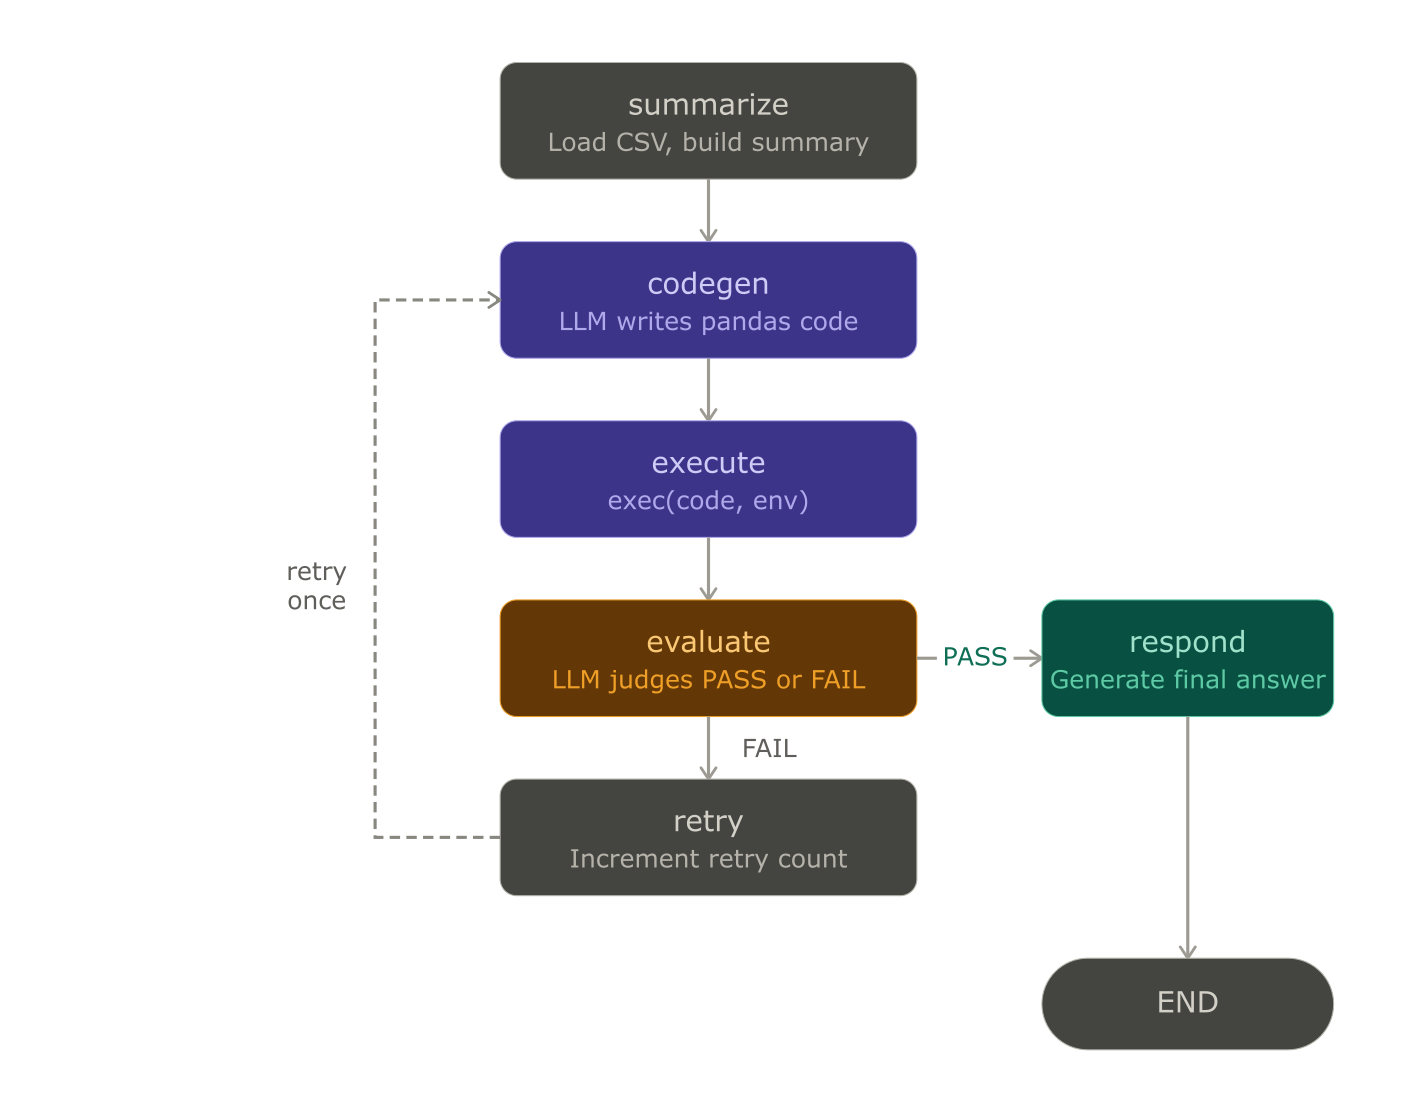
\includegraphics[width=0.8\linewidth]{agent_workflow_diagram.png}
    \caption{Agent Workflow Diagram}
\end{figure}

% ============================================================
\chap{Prompt Log}
% ============================================================

The following prompts were used when building the agent with Claude (claude.ai). Each entry describes what was being attempted and whether the response was helpful.

\subsect{Prompt 1 --- Understanding LangGraph state and nodes}

\textbf{Prompt:} \textit{``I need to build a LangGraph agent in Python. I have not used LangGraph before. How do nodes and state work? What does a basic StateGraph with two nodes look like?''}

\textbf{Goal:} Understand the core LangGraph primitives --- \texttt{StateGraph}, \texttt{TypedDict} state, node functions, and edges --- before writing any project-specific code.

\textbf{Response:} Helpful. The assistant explained that each node is a plain Python function that receives the full state dict and returns a partial dict of keys to update, and that LangGraph merges the returned dict back into state automatically. A minimal two-node example with \texttt{set\_entry\_point} and \texttt{add\_edge} made the pattern clear.

\subsect{Prompt 2 --- Implementing the codegen node}

\textbf{Prompt:} \textit{``Write a codegen node for my agent. It should call OpenAI GPT-5-mini with a system prompt that instructs the model to write pandas code that reads a CSV and stores the result in a variable called \texttt{result}. The node should strip any markdown fences from the output.''}

\textbf{Goal:} Implement the first node of the pipeline, including the system prompt, the OpenAI API call, and fence-stripping post-processing.

\textbf{Response:} Helpful. The assistant produced a clean node function using \texttt{re.sub} to strip fences and a system prompt with explicit rules covering the \texttt{result} variable requirement, the prohibition on \texttt{print()}, and the instruction to return only raw code.

\subsect{Prompt 3 --- Wiring the full graph with retry logic}

\textbf{Prompt:} \textit{``Now add execute, evaluate, and respond nodes, and wire them into a StateGraph in agent.py. The graph should retry codegen once on a FAIL evaluation before falling through to respond.''}

\textbf{Goal:} Complete the four-node pipeline and implement the conditional retry edge using \texttt{add\_conditional\_edges}.

\textbf{Response:} Helpful. The assistant implemented the routing function, a small \texttt{increment\_retry} node to track retry count, and the correct conditional edge mapping.

\subsect{Prompt 4 --- Adding dataset context to improve code generation}

\textbf{Prompt:} \textit{``Let's pass some summary information about the dataset to the LLM calls so that it can create better code. Add a summarize node that reads the CSV once and injects shape, column names, dtypes, first 3 rows, numeric stats, and null counts into the state.''}

\textbf{Goal:} Reduce codegen failures caused by the model inventing incorrect column names or ignoring null values. The summary would be cached per CSV path and passed to both the codegen and respond prompts.

\textbf{Response:} Helpful. The assistant added a \texttt{summarize\_node} function with an in-process \texttt{\_summary\_cache} dict, wired it as the new entry point in \texttt{agent.py}, and updated both prompt templates to include the summary. The retry edge was correctly routed to skip the summarize node (since the summary is already in state), going directly back to codegen.

\subsect{Prompt 5 --- Debugging the genre pairs question}

\textbf{Prompt:} \textit{``This advanced question is failing: 'Identify pairs of genres with similar median income levels but significantly different median house value.' The answer is showing row counts instead of popularity scores in the pair output. How do I fix this?''}

\textbf{Goal:} Diagnose why the generated pandas code was reporting counts alongside genre pair metrics instead of average popularity values, and determine whether the fix should be a prompt change or a question rewrite.

\textbf{Response:} Helpful. The assistant identified that the model was likely including a \texttt{count} column from \texttt{groupby().agg()} output in the final result, which the respond node then misread as a popularity metric. It recommended rewriting the question with explicit numerical thresholds rather than vague qualitative language (e.g.\ ``similar'' and ``significantly different''), which removes ambiguity that causes the model to produce poorly structured output.

\subsect{Prompt 6 --- Refining the genre pairs question with explicit thresholds}

\textbf{Prompt:} \textit{``Rewrite this question with precise thresholds: find genre pairs where average tempo differs by less than 5 BPM and average energy differs by less than 0.05, but average popularity differs by more than 15 points.''}

\textbf{Goal:} Produce a version of the advanced question that the codegen node could implement correctly without ambiguity, yielding a well-structured result the respond node could summarize clearly.

\textbf{Response:} Partially helpful. The rewritten question did fix the codegen bug --- the generated code correctly computed genre-level aggregates and applied the three threshold filters. However, 167 pairs were returned and the respond node listed examples rather than synthesizing patterns across them, making the final answer verbose and hard to interpret.

% ============================================================
\chap{Failure Analysis and Debugging}
% ============================================================

\sect{Failure Case 1 --- Genre Pairs: Count Confused with Popularity}

\textbf{Question:} \textit{Identify pairs of genres with similar average tempo and energy but significantly different average popularity. What other features might explain the popularity gap?}

\textbf{Did the generated code work on the first attempt?} No.

\textbf{What went wrong:} The generated code used \texttt{groupby().agg()} to compute per-genre statistics and included \texttt{count} as one of the aggregated columns (a common pandas pattern). The respond node then interpreted the count column as popularity scores, producing output like ``iranian vs pop-film (counts 38 vs 55)'' --- where 38 and 55 were the number of tracks per genre in the sample, not their average popularity. The actual popularity difference was never computed or reported.

\textbf{How it was debugged:} By inspecting the printed \texttt{execution\_result} in the terminal output, the count/popularity confusion was visible: the numbers were far too small to be popularity scores (which range 0--100) and did not vary enough across genres to explain the stated differences. Comparing the \texttt{generated\_code} output confirmed that \texttt{count} was being passed through to the result DataFrame alongside the actual aggregates.

\textbf{How the prompt was modified:} The question was rewritten with explicit numerical thresholds to remove all qualitative language:

\begin{quote}
\textit{Find genre pairs where average tempo differs by less than 5 BPM and average energy differs by less than 0.05, but average popularity differs by more than 15 points. For each pair, identify which audio features (danceability, acousticness, speechiness, instrumentalness, valence) show the largest differences.}
\end{quote}

\textbf{Did the revised prompt improve the result?} Partially. The codegen bug was resolved --- the revised code correctly computed mean popularity per genre and applied all three threshold conditions. However, 167 pairs met the criteria and the respond node listed individual examples rather than summarizing the dominant pattern across pairs. The answer became more correct but less readable.

\sect{Failure Case 2 --- Housing Coastal Areas: Ambiguous Question Definition}

\textbf{Question:} \textit{Find coastal areas where house prices are relatively low despite proximity to the ocean. What factors might explain this?}

\textbf{Did the generated code work on the first attempt?} Yes, technically --- but the answer was unsatisfying.

\textbf{What went wrong:} The question contains two undefined terms. First, ``coastal areas'' is ambiguous in this dataset: the \texttt{ocean\_proximity} column has categories like \texttt{<1H OCEAN}, \texttt{NEAR OCEAN}, and \texttt{NEAR BAY}, but ``coastal'' could also be interpreted geographically using latitude and longitude to find tracts near the coastline. The generated code chose the categorical interpretation, which is reasonable but not the only valid approach. Second, ``relatively low'' has no threshold --- lower than the dataset average, lower than other coastal categories, or below some absolute value? The code compared \texttt{ocean\_proximity} categories to each other, finding that \texttt{<1H OCEAN} has the lowest average house value among coastal categories (\$213,600), and attributed this to higher population density, household size, and lower room counts.

\textbf{How it was debugged:} The execution result was inspected and the final answer was read carefully. The answer was factually plausible but reflected only one interpretation of the question. No code error occurred; the failure was semantic rather than technical.

\textbf{How the prompt was modified:} A more precise rewrite was proposed:

\begin{quote}
\textit{Among tracts categorized as NEAR OCEAN or NEAR BAY, identify those with median house values below \$200,000. How do their median income, population density, and housing age compare to higher-priced coastal tracts?}
\end{quote}

\textbf{Did the revised prompt improve the result?} This rewrite was not tested in the final run. The original question was retained for the submission and is documented here as a case where question ambiguity, rather than a codegen bug, was the root cause of an unsatisfying answer.

% ============================================================
\chap{Self-Grading}
% ============================================================

\sect{Housing Dataset}

\textbf{Simple questions:} All three are correct and verifiable. The average median house value (\$206,943.86), the identification of ISLAND as the highest ocean proximity category (\$414,700), and the min/max/median statistics (\$14,999 / \$500,001 / \$178,750) can all be confirmed directly from the dataset.

\textbf{Intermediate questions:} All three produced correct, well-structured answers. The median income by ocean proximity question correctly ranked all five categories, included counts, standard deviations, and quartiles, and identified INLAND as a clear outlier on the low end. The geographic binning question used a 10$\times$10 lat/lon grid with a minimum sample count filter (50), which is a sound approach; the top areas correctly correspond to the San Francisco Bay Area and Los Angeles regions. The population density question correctly derived population per household, computed a Pearson correlation ($r = -0.044$), fit a linear model, and reported quantile-grouped means --- a thorough and numerically accurate answer.

\textbf{Advanced questions:} Results were mixed. For the top-5 expensive areas question, the generated code grouped by \texttt{ocean\_proximity} rather than by lat/lon bins. This is accepted as a valid interpretation of the ambiguous term ``geographic area,'' though it differs from the approach used in the intermediate question. The ISLAND result (n=1) is an acknowledged outlier in the answer itself. For the coastal areas question (Failure Case 2), the code and answer are technically correct but semantically limited, as discussed in the failure analysis. For the similar-income/different-value question, the decile-binning approach is reasonable and the identified price ranges are plausible; ISLAND (n=1) inflates the range in the lowest income bin, which the answer itself flags as a potential outlier.

\sect{Spotify Custom Dataset}

\textbf{Simple questions:} All three are correct. Average popularity (32.84), the highest-danceability genre (reggae, 0.768), and the explicit track percentage (8.02\%) are all straightforward aggregations that the agent computed correctly.

\textbf{Intermediate questions:} All three produced strong answers. The energy-by-genre question correctly identified the top 10 most common genres by count and ranked them by average energy, with grindcore (0.938) and black-metal (0.880) at the high end and tango (0.347) at the low end --- a plausible and well-structured result. The tempo-danceability binning question correctly applied the three-bin definition and found that medium-tempo tracks (90--130 BPM) are most danceable on average (0.618), with a clear monotone relationship across bins. The valence-vs-popularity question correctly identified the top-5 genres by valence and noted the nuanced relationship: forró is both high-valence and high-popularity (42.3), while salsa and reggae are high-valence but low-popularity.

\textbf{Advanced questions:} Results were partially correct. For the top-10 popular tracks question, the code correctly identified the tracks, computed feature means and compared them to dataset quartiles, and noted that danceability is the strongest differentiator (50\% of top-10 above the 75th percentile); however, the respond node listed statistics rather than synthesizing a clear pattern, making the answer verbose. For the acousticness/popularity question, the agent filtered at the track level (59 tracks with acousticness $>$ 0.7 and popularity $>$ 60) rather than at the genre level as the question requires --- this is a misinterpretation and the result is marked as a fail. For the genre pairs question (Failure Case 1), the mechanics were correct after the prompt rewrite but 167 pairs overwhelmed the respond node, which listed examples without synthesizing the dominant explanatory feature (instrumentalness) across pairs.

% ============================================================
\chap{Advanced Question Reflection}
% ============================================================

\sect{Housing Dataset --- Advanced Questions}

\subsect{Question 1: Top 5 Most Expensive Geographic Areas}

\textit{Identify the top 5 most expensive geographic areas and explain the key factors contributing to their high prices.}

The generated code interpreted ``geographic area'' as an \texttt{ocean\_proximity} category rather than a lat/lon bin, yielding the five proximity categories ranked by average price: ISLAND (\$414,700), NEAR BAY (\$259,013), NEAR OCEAN (\$254,111), $<$1H OCEAN (\$239,409), and INLAND (\$125,557). This is a valid interpretation of the data, but it is not the only one. A reader could equally expect lat/lon grid cells, ZIP codes, or named cities --- none of which the dataset contains directly. The ISLAND result is also based on a single observation (n=1) and is more likely a data artifact than a meaningful geographic area.

Additionally, ``key factors'' invites causal language. The answer correctly avoids causal claims and instead attributes higher prices to coastal proximity and lower population per household, both of which are correlational findings.

\textbf{Is the answer the only correct one?} No. A lat/lon binning approach (as in the intermediate question) would produce a completely different set of five areas, yet be equally defensible. The question is ambiguous about what constitutes a ``geographic area.''

\textbf{Rewrite:} \textit{Divide the dataset into a 5$\times$5 grid of latitude/longitude bins. Identify the 5 bins with the highest average median house value (requiring at least 30 observations per bin). For each bin, report the average median income, population density, housing age, and ocean proximity distribution, and compare these to the dataset-wide averages.}

\subsect{Question 2: Low-Priced Coastal Areas}

\textit{Find coastal areas where house prices are relatively low despite proximity to the ocean. What factors might explain this?}

The generated code correctly identified $<$1H OCEAN as the lowest-priced coastal category (median \$213,600 vs.\ \$231,900 for NEAR BAY and \$235,100 for NEAR OCEAN) and attributed lower prices to higher population density (3.055 persons/household vs.\ 2.617 for NEAR BAY), larger housing stock (n=4,380), fewer rooms per household (5.142 vs.\ 5.467 overall), and younger housing age (29.35 vs.\ 37.80 for NEAR BAY). These are plausible and data-grounded explanations.

\textbf{Is the answer the only correct one?} No. ``Coastal'' could be defined geographically (latitude/longitude near the coastline) rather than categorically, which could yield a different and finer-grained set of low-priced tracts. ``Relatively low'' also has no threshold --- the agent compared proximity categories to each other, but comparing to the overall dataset median or to an absolute dollar value would both be valid interpretations.

\textbf{Rewrite:} \textit{Among tracts categorized as NEAR OCEAN or NEAR BAY, identify those with a median house value below \$200,000. For each such tract, report the median income, population per household, rooms per household, and housing age, and compare these to the average values for all NEAR OCEAN and NEAR BAY tracts.}

\subsect{Question 3: Similar Income, Different House Values}

\textit{Identify areas with similar median income levels but significantly different median house values. What factors might explain these differences?}

The generated code binned income into deciles and pivoted by \texttt{ocean\_proximity}, revealing large price spreads within income bins driven almost entirely by coastal proximity. In the lowest income bin (\$2.715--3.125k), INLAND median value is \$105,850 while ISLAND is \$414,700 (range \$308,850), though ISLAND's n=1 makes this comparison unreliable. In the highest income bin (\$6.153--15.0k), NEAR OCEAN reaches \$496,150 vs.\ INLAND \$273,800 (range \$222,350). The answer correctly identifies ocean proximity, household crowding, and bedroom-to-room ratio as contributing factors.

\textbf{Is the answer the only correct one?} No. ``Similar'' income and ``significantly different'' values are both undefined --- the decile binning is one valid operationalization, but equal-width bins, quintiles, or a continuous approach using correlation residuals would all produce different pairs. Furthermore, ISLAND (n=1) should arguably be excluded from any comparison.

\textbf{Rewrite:} \textit{Group tracts into five equal-sized median income quintiles, excluding the ISLAND category due to insufficient data. Within each quintile, identify the ocean proximity subcategory with the highest and lowest median house value. For each pair, report the difference in housing age, rooms per household, and population per household.}

\sect{Spotify Dataset --- Advanced Questions}

\subsect{Question 1: Audio Features of Top 10 Popular Tracks}

\textit{Identify the top 10 most popular tracks and analyze what audio features (energy, danceability, valence, tempo) they share. Do popular tracks cluster around specific feature ranges?}

The generated code correctly identified the top 10 tracks (including artists such as Arctic Monkeys, Bad Bunny, Dua Lipa, and Harry Styles) and compared their feature means to dataset quartiles. Key findings: the top-10 mean danceability (0.666) exceeds the dataset median (0.576), with 50\% of top-10 tracks above the 75th percentile for danceability. Energy and valence are close to dataset medians. Tempo ranged widely (67.5--176.1 BPM), indicating no tight cluster. The code's conclusion --- that popular tracks trend toward higher danceability but show no single tight cluster --- is well-supported by the numbers.

\textbf{Is the answer the only correct one?} No. ``Share'' could be interpreted as requiring all 10 tracks to fall within a common range (a stricter definition), or as noting any central tendency (the looser interpretation the agent used). Additionally, the top-10 tracks in a 5,000-row sample may not represent the top-10 in the full 114,000-row dataset.

\textbf{Rewrite:} \textit{Identify the 10 tracks with the highest popularity score. For energy, danceability, valence, and tempo, report the mean and standard deviation for the top-10 group and for the full dataset. For each feature, note whether the top-10 mean falls above the dataset 75th percentile, between the 25th and 75th percentile, or below the 25th percentile.}

\subsect{Question 2: High Acousticness with High Popularity}

\textit{Find genres where high acousticness ($>$0.7) coexists with high popularity ($>$60). What characteristics do these genres share, and what might explain the combination?}

The agent filtered at the track level (59 tracks meeting both thresholds) and then summarized per genre, rather than filtering at the genre level (genres whose average acousticness $>$ 0.7 and average popularity $>$ 60). This is a partial misinterpretation of the question, which asked for genres, not tracks. That said, the genre-level summary produced was informative: singer-songwriter, indian, pop, chill, sad, and indie all appeared with multiple qualifying tracks and high mean popularity (62--72). The shared characteristic of substantially lower loudness (singer-songwriter $-4.07$ dB, chill $-6.40$ dB, sleep $-26.44$ dB below overall mean) is a useful and data-supported finding. The explanation --- that acoustic, intimate arrangements achieve popularity through playlist placement and film/TV sync --- is plausible but goes beyond what the data can confirm.

\textbf{Is the answer the only correct one?} No. Filtering at genre level vs.\ track level produces different results, and the interpretation of ``characteristics'' could be restricted to dataset columns only (stricter) or extended to cultural and industry explanations (as the agent did).

\textbf{Rewrite:} \textit{Compute the average acousticness and average popularity for each genre. Identify genres where average acousticness exceeds 0.7 and average popularity exceeds 60. For each qualifying genre, report average danceability, valence, speechiness, instrumentalness, and loudness. If no genres meet both thresholds, relax the popularity threshold to 50 and note the change.}

\subsect{Question 3: Genre Pairs with Similar Tempo and Energy but Different Popularity}

\textit{Find genre pairs where average tempo differs by less than 5 BPM and average energy differs by less than 0.05, but average popularity differs by more than 15 points. For each pair, identify which audio features (danceability, acousticness, speechiness, instrumentalness, valence) show the largest differences.}

The generated code correctly computed per-genre means, applied all three threshold conditions, and iterated over all genre combinations. The mechanics are correct. However, 167 pairs met the criteria, and the respond node listed 10 examples rather than synthesizing the dominant pattern. Examining the results, instrumentalness is the top-differentiating feature in the majority of high-popularity-gap pairs (e.g., iranian vs.\ pop-film: 0.459, iranian vs.\ k-pop: 0.432, idm vs.\ pop-film: 0.681), suggesting that instrumental content is a key driver of the popularity gap when tempo and energy are matched. This cross-pair pattern was not surfaced in the final answer.

\textbf{Is the answer the only correct one?} No. 167 pairs is itself ambiguous --- a stricter popularity threshold (e.g., $>$ 20 points) would reduce this to a more interpretable set. The choice to show only 10 examples, sorted by popularity difference, means the answer is a valid subset but not a complete or synthesized result.

\textbf{Rewrite:} \textit{Find all genre pairs where average tempo differs by less than 5 BPM and average energy differs by less than 0.05, but average popularity differs by more than 20 points. Across all qualifying pairs, compute the average absolute difference for each of the five audio features (danceability, acousticness, speechiness, instrumentalness, valence). Report which feature shows the largest average difference, then list the top 5 pairs ranked by popularity gap.}
\end{document}
